\documentclass{article}
\usepackage[UTF8]{ctex}
\usepackage{geometry}
\usepackage{multirow}
\usepackage{natbib}
\geometry{left=3.18cm,right=3.18cm,top=2.54cm,bottom=2.54cm}
\usepackage{graphicx}
\pagestyle{plain}
\usepackage{float}	
\usepackage{setspace}
\usepackage{enumerate}
\usepackage{caption2}
\usepackage{datetime} %日期
\renewcommand{\today}{\number\year 年 \number\month 月 \number\day 日}
\renewcommand{\captionlabelfont}{\small}
\renewcommand{\captionfont}{\small}
\begin{document}

\begin{figure}
    \centering
    
\includegraphics[width=8cm]{upc.png}

    \label{figupc}
\end{figure}

	\begin{center}
		\quad \\
		\quad \\
		\heiti \fontsize{45}{17} \quad \quad \quad 
		\vskip 1.5cm
		\heiti \zihao{2} 《计算科学导论》个人职业规划
	\end{center}
	\vskip 2.0cm
		
	\begin{quotation}
% 	\begin{center}
		\doublespacing
		
        \zihao{4}\par\setlength\parindent{7em}
		\quad 

		学生姓名:\underline{\qquad  张航 \qquad \qquad}

		学\hspace{0.61cm} 号:\underline{\qquad 1907010218\qquad}
		
		专业班级:\underline{\qquad 计算1902 \qquad  }
		
        学\hspace{0.61cm} 院:\underline{计算机科学与技术学院}
% 	\end{center}
		\vskip 1.5cm
		\centering
		\begin{table}[h]
            \centering 
            \zihao{4}
            \begin{tabular}{|c|c|c|c|c|c|c|c|c|}
            % 这里的rl 与表格对应可以看到,姓名是r,右对齐的;学号是l,左对齐的;若想居中,使用c关键字。
                \hline
                \multicolumn{5}{|c|}{分项评价} &\multicolumn{2}{c|}{整体评价}  & 总    分 & 评 阅 教 师\\
                \hline
                自我 & 环境 & 职业 & 实施 & 评估与 & 完整性 & 可行性 &\multirow{2}*{} &\multirow{2}*{}\\
                分析& 分析& 定位 & 方案 & 调整 & 20\% & 20\% & ~&~ \\\            
                10\% & 10\% & 15\% & 15\% & 10\% & &  &~ &~\\
                \cline{1-7} 
                & & & & & & & ~&~ \\
                & & & & & & & ~&~ \\
                \hline      
            \end{tabular}
        \end{table}
		\vskip 2cm
		\today
	\end{quotation}

\thispagestyle{empty}
\newpage
\setcounter{page}{1}
% 在这之前是封面,在这之后是正文
\section{自我分析}
	\par
\subsection{自然条件}
我是来自计算机科学与技术学院,计算机科学与技术专业,计算1902班的张航。性别男。在2000年4 月1 日来到这个世界,至今已经二十年了。\par 
身体条件:身高170的我在男生中算是低的了,体重120斤到还算是在正常范围之内的。对一个当代大学生而言,身体素质无疑也是一道门槛。身体素质不算太好。\par 
健康状况:健康状况良好,从小到大也没生过什么大病,健康状况自我认为还是蛮好的。\par 
学习城市:山东省青岛市。\par 
居住城市:河南省南阳市邓州市\par 
自身对于计算机领域的了解状况:在来大学之前对于计算机领域的了解几乎为零,从来不玩电脑的我甚至连电脑的基本操作都不会,开学到现在经过了一个学期,对于电脑的一些基础知识还是有所了解了。虽然不多,但我接下来还是会尽力去学习尽可能多的关于本专业方面的知识。\par
\subsection{性格分析}
1、性格的态度特征:我的性格是比较理智的类型。我的性格比较实诚、正直。个人感觉还是比较谦虚的。在做事情的时候不认真勤奋责任心强,但自己的创新意识并不强,因此需要多多培养自己的创新思维。但在平时与别人相处时还是比较胆怯,不敢同陌生人交流,只有在熟悉之后才敢说话。\par
2、性格的情趣特征:我的性格感觉还是比较容易冲动的,但是还是比较胆怯的。可能也就是因为胆怯的原因吧,虽然会冲动,但也还是都能控制自己的行为。情绪波动还是比较大的。\par
3、性格的意志特征:我的性格在意志方面是比较顽强、倔强、不会轻易放弃的,但是有点优柔寡断,遇事经常会犹豫不决,这可能是一个极大的缺点吧。我会尽可能克服这个缺点,让自己变的更加果断。同时,在对事物的预知上是属于乐观但同时有比较强的忧患意识,而且充满了对于未知事物的害怕。不仅如此,我还经常会害怕自己落后,跟不上不上大家的脚步。可能这也是一种自卑心理吧。我会尽可能克服这种心理,努力做到谦虚但又不自卑。做一个更好的自己。\par
4、性格的理智特征:在感知注意方面,我是属于那种不太喜欢主动观察的类型。在想象方面,我是属于那种想象力丰富的类型,经常沉浸在自己的世界里。或许是因为内向的性格吧,不太喜欢说话,因此沉浸在自己的世界里的时间可能就格外多了吧。虽然说这种性格可能很适合一个程序员,但是我还是会尽可能地去和别人交流,毕竟,合作交流才能进步,性格开朗才能交到更多知心的朋友。才能拥有更多的交流与快乐。\par
\subsection{教育与学习经历}
我的教育与学习经历平平,没有在其中得到过什么荣誉,然而也并没有受到过什么处罚。\par
幼儿园时期:自从四岁进入那个离家里不算太远的幼儿园,我的人生直到现在便都是在学习的路上一去不复返。幼儿园的生活不算太快乐,但也不算多难过,就这么平平淡淡地过去了。\par 
小学时期:从幼儿园到村里的小学。小学可以算得上是一段先苦后甜的日子了,从开始一二三年级的时候因为背不过课文被留校,又到因为学习成绩太差而被留级,或许正是因为这些,才让我在小学接下来的日子里努力学习,努力去使自己变得不再那么差劲。
初中时期:从小学进入镇上的初中,我又落回了后边。毕竟初中时候我面对的人更多,也都更优秀,而我在他们之中又变得落后了许多。于是,一样不服输的心,一样为了使自己能够不再差劲,又是一段一样的拼搏,努力的前进。\par 
高中时期:高中时期算是比较关键的时期了,毕竟,高考越来越近了,面对着这一重大人生节点,没人再敢放松。每一次升学,都是离家越来越远。头一次半个月回家一次,竟没有什么不适应。或许是学习的忙碌吧。\par 
大学时期:现在的我正就读于中国石油大学,经过了高中,才知道时间可以过的多么快。在大学里,要掌握的知识也变得多起来了,学习也越来越忙,毕竟,知识越来越难学,也越来越多。目前在大学也已经过去了一个学期,也算是逐渐适应了大学生活。自己目前掌握的知识并不多,但是大学还有三年半,这三年半也是人生重要的知识掌握时期。我会尽我所能,去掌握尽可能多的知识,尽力去接受更高的教育。\par
\subsection{工作与社会阅历}
关于工作经历方面,毕竟到现在还是学生,因此工作经历并不多,可是称得上是工作经历的只有各种寒暑假的暑假工了吧。从小到大,我只在高一的暑假期间做过一次暑假工。高一暑假在我新乡的二姨家里住,并在哪里找了一份暑假工作,是在一家酒店里做传菜员。真的是不当家不知柴米油盐贵,真正干起活来,才知道挣钱有多难。通过这一次暑假工的经历,我明白了社会的现实,每个人都不容易,挣钱养家真的挺难。这次之后就因种种原因而没有干过暑假工。而且由于一直呆在学校,社会阅历方面也十分贫乏,或许只有那一次的暑假工经历才能算得上社会阅历吧。\par
\subsection{知识、技能与经验}
关于知识掌握方面,只有从小学到现在的在学校所得到的知识。技能方面因为一直沉浸于学习,也并没有掌握什么特别的技能。今后如果有时间可能会有这方面的兴趣,会培养自己拥有几个技能。经验就目前而言,掌握的大多数还是学习方面的经验和一些生活经验。\par
\subsection{兴趣爱好与特长}
我最大的兴趣爱好就是学习。之前因为条件有限,也可能的是因为自己的原因,并没有什么太感兴趣的事情,但自从上了大学之后,我发现我对乒乓球、羽毛球和排球还是比较有兴趣的,今后也会更加喜欢这几项。我感觉就目前而言,我的特长还是羽毛球,因为羽毛球算是从小就接触的运动了,我打的还是不错的。\par
\section{环境分析}
\par
\subsection{社会环境分析}
1、政治形势:目前社会对于计算机行业还是比较认可的。目前国家也比较支持计算机行业的发展,毕竟属于高科技行业,对计算机行业政策上也有所照顾,这是计算机行业得以发展迅速的根本原因。\par 
2、经济形势:目前计算机行业所创造的经济总值已经位居前列,成为了经济增长的重要一极。\par 
3、就业形势:目前计算机行业的就业形势十分乐观,社会上计算机行业的人才缺口依旧很大,计算机行业的职位工作待遇一般都是比较好的。毕竟,计算机行业未来必定是一重要行业,而现在人才缺口又比较大,因此目前计算机行业的就业形势是一片大好。\par
\subsection{家庭环境分析}
家庭环境很温馨,不过我至今还是单身。家庭经济状况不算太好也不算太坏。家庭不算太富裕,但父母也都在为生活而努力。家人自然是期望我能好好读书,将来出去能够找一份好工作,能够帮助家庭分担一些负担,能够安安稳稳地生活。这也是我努力学习新知识的动力之一。\par
\subsection{职业环境分析}
关于行业:计算机行业目前发展态势良好,劲头正足。现在的社会,计算机技术几乎渗透到了各个行业,因此,计算机在未来几乎是必不可少的存在,因此计算机行业的人才几乎都能得到很好的发展。在未来,计算机行业必然会渗透到社会各个方面,发展前景几乎是不容置疑的好。目前来看,能够威胁到计算机行业发展的,根本不会有。\par 
关于职业:我未来理想的职业是是软件开发工作者。该职业主要的工作内容就是进行软件的开发与测试。并在公司要求下进行系统的开发与维护。而这个职位的工作要求,自然要有耐得住寂寞,能看得下去那些多的很的代码的耐心。更要有必要的基础知识的支撑。\par 
发展前景:就目前的形势来看,有关计算行业的职位的待遇都不会差。而且软件开发这一个职位未来肯定会有一片独特的天地。现在的社会智能化发展日益加快,因此,对于由各种软件控制的智能的需求必然会以指数般的速度增长,而这,就是软件开发工作者未来的黄金时期。\par
\begin{figure}[H]
	\centering
	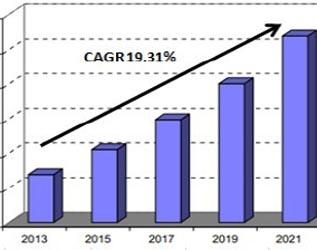
\includegraphics[scale=1.0]{jisuanjifazhanqushi}
	\caption{计算机发展趋势}
	\label{fig:jisuanjifazhanqushi}
\end{figure}

\subsection{地域与人际环境分析}
我理想的工作城市是在上海。毕竟是大城市,将来机会会比较多,而且离家里还算是比较近的。上海的气候温和,没有太冷的日子,也没有太热的日子,个人感觉还是挺适宜居住的。\par 
文化特点:上海也算是一座比较典型的移民城市,在这里可以体会到东西方文化的交融,上海的多元与包容。上海的历史就是在东西方的交融中进行的,也算是世界的一个交流中心。\par 
发展前景:上海毕竟是一个大都市,未来在智能化方面的发展肯定会有极大的力度,因此在上海,计算机行业可以说是很有前景的了。除了政策上的支持,上海还是一个都市,因此能够做到与世界上先进技术的交流,从而更多地促进自身的发展。\par 
人脉:关于在上海的人脉这一方面,我并没有什么优势,毕竟家里也没人在外面面发展过,尤其是在这一个行业。但是,人脉是可以自己建立的,毕竟不是所有人一出来就有很好的人脉,我会尽量去结交朋友,以使自己在这个陌生的城市拥有属于自己的人脉圈。\par
\par \par



\section{职业定位}
\par

\subsection{行业领域定位与理由}
对我而言,我将来想要从事的当然是计算机行业了。至于原因,最重要的一点,也是我选择这个专业的原因当然是将来这个行业还是比较容易就业的。再次,这个行业的工资还算可以,虽然可能工作会很累,有点拿命挣钱的感觉,但是在这个世界上,谁又不是在拼命地挣钱以求能过上一个好一点的生活呢。我也不说对这个行业将来会有多大的贡献,但我会尽自己所能去完成自己应该做的事情。\par
\subsection{职业岗位起点定位与理由}
职业方面的话,上面已经提到了,我理想的职业是一名软件开发工作者。我的职业岗位起点定位并不高,只希望能够进一个好点的公司,先做一个小的职业工作者也好。毕竟路是一点一点走的。在计算机这个行业,经验往往是最重要的。因此,从小处入手,逐步积累,才能为之后大的突破积聚力量。\par
\subsection{职业目标与可行性分析}
\par
\par 
\begin{enumerate}[(1)]
	\item 短期目标(大学4年)\par 
	短期目标当然是在大学期间好好学习,不落后,不拖沓,尽量去掌握尽可能多的知识,充实自己的大脑,多多向别人学习,学会问问题,当然也要学会自主解决问题。\par 
	\item 中长期目标(5-10年)\par 
	对于未来毕业后五到十年间的目标,目前的打算是先要读研究生,这三年期间肯定是艰苦的三年,毕竟这时候才开始能知道自己之前学的大多数知识真正的用途。研究生研究生,顾名思义,肯定是要做研究的。所以在研究生期间一定要认真做研究,认真学习各种知识。至于之后,肯定是要考虑工作问题。我想我对于工作不会太挑剔,只要工资能够满足日常生活所需就可。入职的前两年,是积累经验的时间。这时候作为一个职场小白,对于在工作中出现的各种问题的处理能力相对不到位,这便是学习的意义所在。在经过了两年的磨练,对于自己工作的事务也开始熟悉起来,这时候,就可以开始尝试去寻找一些自己所期望的公司。去尽力的加入他们,并努力做好自己的本职工作,并在工作之外的时间不断学习,充实自己,以避免被淘汰。这时候就可以适当提高自己的工资标准,去争取一些工资较高的岗位。但我感觉,就我个人而言,可能还是更适合于研发型岗位,不太喜欢也不太愿意去做管理层,因此,可能会更加倾向于技术型岗位。\par 
	
\end{enumerate}



\section{实施方案}
在明确了职业定位后,要制定实现职业生涯目标的行动方案,不付诸行动,职业目标只能是一种梦想。实施方案是实现职业目标的保证,尽量考虑周全、具有可操作性。\par
实施方案可以从以下角度考虑:\par
\begin{enumerate}[1、]
	\item 如何利用现有条件和自身优势以实现职业生涯目标:\par 
	现有条件:对于我理想的工作岗位来说,在现有条件方面,我感觉我拥有的更多的是如今的学习条件,因此我会充分利用学校图书馆与自习室等资源去提升自己,去使自己能够更加接近自己的目标。\par 
	自身优势:我觉得我唯一的优势可能就是比较耐心,在研发过程中可能会很好地进行检查,尽量去达到使自己满意的程度。\par 
	\item 如何克服缺点、弥补不足、增长知识、提高能力以实现职业生涯目标:\par 
	我会克服自己的胆怯,积极主动去和别人交流,去探讨问题,而不是自己一个人闷头自己搞。毕竟,闭门造车是不行的,只有主动与别人交流,才能知道自己哪里不足,才会知道别人曾经在那里出过错,再次遇到的时候就会小心避免出错,只有这样才能进步。\par 
	\item 如何处理人际关系和发展人脉以实现职业生涯目标:我对于人与人之间的交流方面太过薄弱,内向的性格使得我不太善于与人交流。但我会努力克服自己,给自己积极的心理暗示,告诉自己要努力与人交流,多与人交朋友,多交知心朋友,使自己的人脉圈更大,以便更好地发展。\par 
	\item 如何处理工作与家庭、生活的关系以实现职业生涯目标:\par 
	工作的压力与家庭生活之间的矛盾不然会存在,全身心投入工作必然忽略家庭。因此,需要更好的与家人沟通,争取获得理解。但自身也不能真的没有行动。给自己定一个目标,在多长的时间里同家人一起出去旅游放松,每天抽出一定的时间同家人聊聊天,多陪陪家人。未尝不是一种解决这个问题的好方法。关键在于不找客观理由,自己真正真心的去做。\par 
	\item 如何处理释放工作压力、保证身心健康以实现职业生涯目标:\par 
	在现代社会,工作压力难以避免,因此,过于严重的工作压力会对人造成很严重的伤害,因此,如何释放压力也很重要。我感觉,释放压力最好的措施,便是让自己出去疯玩一次,工作的时间久了,难免有压力,这时候出去玩一趟,完全忘掉工作,难道不是一种很好的减压方法吗?另外,我还会多找些知心的朋友去倾诉,当然,也会和家人诉说一番,这不失也是一种很好的方法。
\end{enumerate}
\par 

\section{评估与调整}\par 
\subsection{评估时间}
中国儒家经典《礼记·大学》中说过“苟日新,日日新,又日新”。因此,我们应当经常对自己的目标也做些审视。不用太短,也不能太长。一个学期无疑是最好的时间。一个学期的结束,意味着一段学习时间的结束,也正好有时间来对这段时间的形势变化做一个分析,并对自己的规划做一个调整。\par
\subsection{评估内容}
评估的内容当然是自己规划之中所要达到的各种目标,比如对自己预期工资的调整,对自己所要拥有的能力的调整。这些都是会随着时间而发生变化的。因此,经常性的调整才能使自己更好地按照自己所规划的目标继续前行。\par
\subsection{调整原则}
在调整的时候,我会考虑多方面因素。多与自身目前的实际情况、预期工作地点的的行业环境变化以及更改的规划的可行性方面考虑,考虑一定要周到。以便我在规划的实施过程中可以顺利进行。\par




\end{document}
